\documentclass[10pt]{beamer}
\usetheme{Madrid}
\usepackage{booktabs}
\usepackage{graphicx}
\usepackage[T1]{fontenc}
\usepackage{tikz}
\usetikzlibrary{arrows.meta}
\setbeamertemplate{navigation symbols}{}
% To view speaker notes, uncomment the next line (adds note pages):
% \setbeameroption{show notes}
\tikzset{
  box/.style={draw, rounded corners, align=center, text width=2.3cm, minimum height=0.9cm, font=\scriptsize},
  kuser/.style={box, fill=blue!15}, kagent/.style={box, fill=green!25},
  kdata/.style={box, fill=black!8}, kdanger/.style={box, fill=red!25},
  koutput/.style={box, fill=orange!25}, kdecision/.style={box, fill=yellow!30},
  kguard/.style={box, fill=violet!25},
  flow/.style={-{Stealth[length=2mm]}, thick},
}
% ======================= EDIT YOUR DETAILS =======================
\newcommand{\studentname}{Aflah Muhammed P}
% Change the university roll/registration number:
\newcommand{\rollno}{TVE23CSXXX}
% Change your class roll number:
\newcommand{\rollclass}{Roll No: XX}
% Change your guide name:
\newcommand{\guidename}{Prof. Guide Name}
% Change department / college / short-institute if needed:
\newcommand{\deptname}{Department of Computer Science and Engineering}
\newcommand{\collegename}{College of Engineering Trivandrum}
\newcommand{\shortinst}{CET}
% Change the seminar date:
\newcommand{\seminardate}{\today}
% =================================================================
\title[B.Tech Seminar]{Humans in the Loop: How People and LLM Agents Work Together (A Survey of LLM-HAS)}
\subtitle{Based on: LLM-Based Human-Agent Collaboration and Interaction Systems: A Survey (arXiv:2505.00753, 2025)}
\author[\studentname\ (\shortinst)]{\studentname \\ \small \rollno \\ \small \rollclass \\ \small Guide: \guidename}
\institute[]{\deptname \\ \collegename}
\date{\seminardate}
\begin{document}
\begin{frame}[plain]
  \titlepage
\end{frame}
\begin{frame}{Table of Contents}
  \tableofcontents
\end{frame}
\section{Introduction}
\begin{frame}{Introduction}
\begin{itemize}
  \item LLM agents are AI programs that plan and act on their own.
  \item Fully autonomous agents still hallucinate and make unsafe mistakes.
  \item Adding a human in the loop boosts reliability, safety, and trust.
  \item This paper is the first structured survey of human-agent systems.
  \item It organizes the field into five clear building blocks.
  \item Goal today: understand how people and agents collaborate well.
\end{itemize}
\end{frame}
\note{Let's start with the big picture. LLM agents are AI systems that can plan and take actions on their own, but on their own they still make things up and can act unsafely. This paper argues the fix is keeping a human in the loop, and it is the first survey to organize how that is done into five clean building blocks.}
\section{Literature Survey}
\begin{frame}{Literature Survey / Background}
  \small
  \begin{tabular}{@{}p{2.7cm}p{2.3cm}p{5.6cm}@{}}
    \toprule
    \textbf{Title} & \textbf{Author} & \textbf{Summary} \\
    \midrule
    MetaGPT: Multi-Agent Collaborative Framework & Hong et al., 2024 & Assigns human-like roles to multiple LLM agents so they cooperate on software tasks with shared standard operating procedures. \\
    \addlinespace
    Training Language Models with Human Feedback (RLHF) & Ouyang et al., 2022 & Uses human preference ratings to fine-tune models, showing feedback makes outputs more helpful, honest, and safe. \\
    \addlinespace
    SOTOPIA: Social Intelligence Evaluation for Agents & Zhou et al., 2024 & Benchmarks how language agents interact socially with humans and each other across cooperative and competitive goals. \\
    \addlinespace
    \bottomrule
  \end{tabular}
\end{frame}
\note{Before this survey, several works pointed the way. MetaGPT showed multiple agents can play human-like roles and cooperate. RLHF proved that human feedback makes models safer and more helpful. SOTOPIA gave us a way to test how socially well agents interact. This paper pulls those threads into one framework.}
\section{Motivation}
\begin{frame}{Motivation}
\begin{itemize}
  \item Autonomous agents fail on complex, high-stakes real-world tasks.
  \item Hallucinations make fully independent agents hard to trust.
  \item Humans add judgment, context, and safety oversight agents lack.
  \item Prior surveys focused on autonomy, not the human side.
  \item Teams and industry need clear patterns for collaboration.
\end{itemize}
\end{frame}
\note{Why care? Because fully autonomous agents break down on complex, high-stakes tasks and can hallucinate confidently. Humans bring judgment, context, and oversight that agents lack. Earlier surveys focused on making agents more independent, but this one focuses on the human side, which is what industry actually needs.}
\section{Problem Statement}
\begin{frame}{Problem Statement}
  \begin{block}{}
  Fully autonomous LLM agents are unreliable and risky for real deployment, yet the field lacks a unified view of how humans should be involved. This survey asks how to structure human information, feedback, and control so agent systems become more reliable, capable, and safe.
  \end{block}
\end{frame}
\note{Here is the core problem in one line. Autonomous agents are not reliable enough to trust alone, and the field had no shared map of how to involve people. The survey asks a simple question: how do we structure human input so systems become more reliable, capable, and safe?}
\section{Objectives}
\begin{frame}{Objectives}
\begin{itemize}
  \item Define LLM-based Human-Agent Systems (LLM-HAS) clearly.
  \item Provide the first structured taxonomy of the field.
  \item Break systems into five core reusable components.
  \item Catalog feedback, interaction, orchestration, and communication choices.
  \item Map applications, tools, and benchmarks across domains.
  \item Highlight open challenges and future research directions.
\end{itemize}
\end{frame}
\note{The authors set out to do a few things. First, clearly define what a human-agent system is. Then build the first structured taxonomy, break it into five reusable components, and catalog the design choices. Finally, map real applications and benchmarks, and flag what is still unsolved.}
\section{Methodology}
\begin{frame}[allowframebreaks]{Methodology: Setting the Stage: Environment, Profiling, and Feedback}
\begin{itemize}
  \item Environment is the shared space, physical or fully simulated.
  \item Profiling defines roles, goals, and agent skills like memory.
  \item Feedback types: evaluative, corrective, guidance, and implicit.
  \item Feedback timing: setup, during task, or post-task.
  \item Feedback granularity: whole-output (coarse) or segment-level (fine).
\end{itemize}
\end{frame}
\note{Now the how. Think of it in three parts. First, set the stage: the environment, the roles of each player, and the kind of feedback humans give. Second, working together: whether they collaborate, compete, and who acts when. Third, staying in sync: how information actually flows between them. I'll walk through each on the next slides.}
\begin{frame}[allowframebreaks]{Methodology: Working Together: Interaction Types and Orchestration}
\begin{itemize}
  \item Collaboration covers delegation, supervision, cooperation, coordination.
  \item Competition and coopetition capture conflicting or mixed goals.
  \item Task strategy: one-by-one turns or simultaneous parallel work.
  \item Temporal sync: synchronous real-time or asynchronous delayed.
  \item Orchestration decides who acts, when, and in what order.
\end{itemize}
\end{frame}
\begin{frame}[allowframebreaks]{Methodology: Staying in Sync: Communication Structures and Modes}
\begin{itemize}
  \item Structure can be centralized, decentralized, or hierarchical.
  \item Centralized has one coordinator; decentralized is peer-to-peer.
  \item Modes: conversation, observation, or a shared message pool.
  \item Conversation uses natural language; observation reads user behavior.
  \item Shared pool is a common repository all parties read.
\end{itemize}
\end{frame}
\section{Key Concepts}
\begin{frame}[allowframebreaks]{Key Concepts}
  \begin{description}
    \item[LLM-HAS] LLM-based Human-Agent System: humans and AI agents working together on a shared task.
    \item[Human-in-the-loop] Keeping a person involved to guide, check, or correct the agent's actions.
    \item[Human Feedback] Signals people give agents: ratings, edits, instructions, or inferred behavior cues.
    \item[Interaction Type] How human and agent relate: collaborate, compete, or a mix of both.
    \item[Orchestration] Coordinating who acts when, in sequence or in parallel, over time.
    \item[Communication] How information flows: structure (centralized, hierarchical) and mode (chat, observation).
  \end{description}
\end{frame}
\note{Let me define the jargon so nothing trips you up. LLM-HAS just means humans and AI agents working together. Human-in-the-loop means a person stays involved to guide or correct. Feedback is any signal you give the agent. Interaction type is your relationship, orchestration is timing, and communication is how you talk.}
\section{System Architecture}
\begin{frame}{System Architecture}
  \begin{center}
  \resizebox{0.96\textwidth}{!}{%
  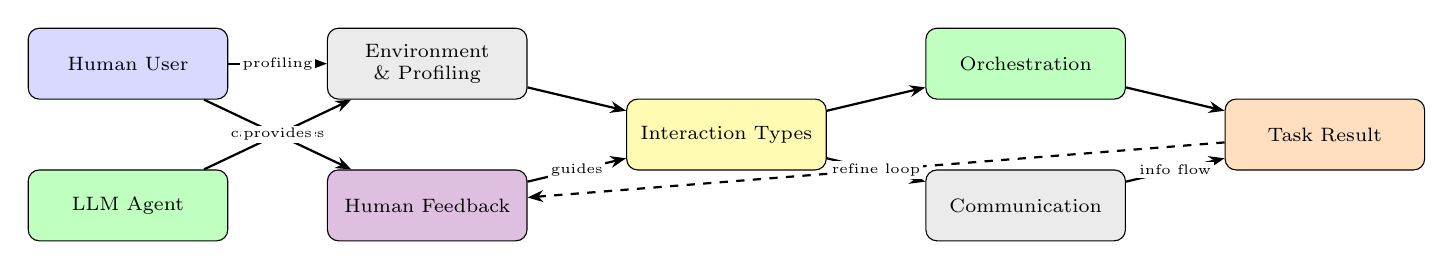
\begin{tikzpicture}
    \node[kuser] (user) at (0.00,0.90) {Human User};
    \node[kagent] (agent) at (0.00,-0.90) {LLM Agent};
    \node[kdata] (env) at (3.80,0.90) {Environment \& Profiling};
    \node[kguard] (feedback) at (3.80,-0.90) {Human Feedback};
    \node[kdecision] (interact) at (7.60,0.00) {Interaction Types};
    \node[kagent] (orch) at (11.40,0.90) {Orchestration};
    \node[kdata] (comm) at (11.40,-0.90) {Communication};
    \node[koutput] (output) at (15.20,0.00) {Task Result};
    \draw[flow] (user) -- (env) node[midway, font=\tiny, fill=white, inner sep=1pt]{profiling};
    \draw[flow] (agent) -- (env) node[midway, font=\tiny, fill=white, inner sep=1pt]{capabilities};
    \draw[flow] (user) -- (feedback) node[midway, font=\tiny, fill=white, inner sep=1pt]{provides};
    \draw[flow] (env) -- (interact);
    \draw[flow] (feedback) -- (interact) node[midway, font=\tiny, fill=white, inner sep=1pt]{guides};
    \draw[flow] (interact) -- (orch);
    \draw[flow] (interact) -- (comm);
    \draw[flow] (orch) -- (output);
    \draw[flow] (comm) -- (output) node[midway, font=\tiny, fill=white, inner sep=1pt]{info flow};
    \draw[flow, dashed] (output) -- (feedback) node[midway, font=\tiny, fill=white, inner sep=1pt]{refine loop};
  \end{tikzpicture}%
  }
  \end{center}
  \begin{center}\scriptsize The LLM-HAS loop: humans and agents interact through five core components to produce refined results.\end{center}
\end{frame}
\note{This diagram is the whole paper in one picture. On the left, a human and an agent both enter, and they configure the environment and profiling. The human also feeds in guidance through the feedback block. That shapes how they interact, which drives orchestration and communication, producing a result. Notice the dashed arrow looping the result back as new feedback.}
\begin{frame}[allowframebreaks]{How It Works (Explained)}
\begin{itemize}
  \item Left side: a human user and an LLM agent both enter the system.
  \item They feed the Environment and Profiling block that sets context, roles, and goals.
  \item The human separately supplies Human Feedback, acting as a safety guide.
  \item Environment and feedback together drive the Interaction Types decision block.
  \item Interaction feeds Orchestration (who acts when) and Communication (how they exchange info).
  \item Both produce a Task Result, which loops back dashed as refining feedback.
\end{itemize}
\end{frame}
\section{Example Walkthrough}
\begin{frame}[allowframebreaks]{Example Walkthrough: A coding assistant fixing a bug, with you in the loop}
\begin{enumerate}
  \item You set the goal: fix a failing function (initial-setup feedback).
  \item Profiling: the agent is a coding expert; you are the reviewer.
  \item The agent proposes a code edit and runs the tests.
  \item A test fails, so the agent shows you the error (communication).
  \item You give corrective feedback: point to the wrong line (fine-grained).
  \item The agent revises synchronously and the tests now pass.
  \item You approve the final result; loop ends with post-task confirmation.
\end{enumerate}
\end{frame}
\note{Let's make it concrete with a coding example. You ask the assistant to fix a failing function. It proposes an edit and runs the tests, but one fails, so it shows you the error. You point to the exact wrong line, it revises, and the tests pass. You approve. That whole cycle is a human-agent system in action.}
\section{Results}
\begin{frame}[allowframebreaks]{Results / Findings}
\begin{itemize}
  \item First comprehensive, structured survey of LLM-HAS.
  \item Organizes the field into 5 core components.
  \item Defines 4 human feedback types across 3 timing phases.
  \item Catalogs 6 interaction types spanning collaboration, competition, coopetition.
  \item Covers 5 application domains and 20+ benchmarks in 3 tables.
  \item Highlights 3 implementation frameworks: Collaborative Gym, CowPilot, DPT-Agent.
\end{itemize}
\end{frame}
\note{So what did the survey deliver? It is the first structured overview of this space, organized into five core components. It defines four feedback types across three timing phases, six interaction types, and covers five application domains with over twenty benchmarks. It also highlights three ready-to-use frameworks like Collaborative Gym.}
\section{Discussion}
\begin{frame}{Discussion}
\begin{itemize}
  \item Structured human involvement measurably improves reliability and safety.
  \item Choice of feedback type trades user effort against signal quality.
  \item Domain shapes the best interaction and orchestration pattern.
  \item A shared vocabulary lets researchers compare systems fairly.
\end{itemize}
\end{frame}
\note{The takeaway is that structured human involvement genuinely improves reliability and safety. But every choice is a trade-off: richer feedback like direct edits costs the user more effort. And the right pattern depends on the domain. Most importantly, a shared vocabulary now lets researchers compare systems fairly.}
\section{Challenges}
\begin{frame}{Limitations \& Challenges}
\begin{itemize}
  \item Human behavior varies widely, resisting standardized frameworks.
  \item Most work is agent-centered, not truly bidirectional.
  \item Evaluation often ignores human effort and workload metrics.
  \item Safety, robustness, and privacy remain underexplored.
\end{itemize}
\end{frame}
\note{Be honest about the gaps. Humans are unpredictable, which makes standardizing hard. Most work still centers the agent, not a true partnership. Evaluations rarely measure how much effort the human spends, and safety, robustness, and privacy are still underexplored.}
\section{Future Work}
\begin{frame}{Future Work}
\begin{itemize}
  \item Build two-way guidance where agents also help humans.
  \item Create metrics that measure human workload and experience.
  \item Strengthen safety, robustness, and privacy protections.
  \item Extend to healthcare, science, and education domains.
\end{itemize}
\end{frame}
\note{Looking ahead, the exciting directions are two-way guidance where the agent also helps the human, and better metrics that capture human workload. There is also a clear call to strengthen safety and privacy, and to bring these systems into healthcare, science, and education.}
\section{Conclusion}
\begin{frame}{Conclusion}
\begin{itemize}
  \item Fully autonomous agents are not yet reliable enough alone.
  \item Adding humans in the loop improves trust and performance.
  \item Five components give a shared map of the design space.
  \item This survey is a foundation for building better human-agent teams.
\end{itemize}
\end{frame}
\note{To wrap up: autonomous agents alone are not ready for prime time, but adding a human in the loop makes them more trustworthy and capable. The five components give us a shared map of the design space. Treat this survey as a foundation for building better human-agent teams.}
\section{References}
\begin{frame}[allowframebreaks]{References}
  \footnotesize
  \begin{enumerate}
    \item Zou, H. P., Huang, W.-C., Wu, Y., Guo, J., et al. (2025). LLM-Based Human-Agent Collaboration and Interaction Systems: A Survey. arXiv:2505.00753. Findings of ACL 2026.
    \item Hong, S., Zheng, X., Chen, J., et al. (2024). MetaGPT: Meta Programming for a Multi-Agent Collaborative Framework. ICLR 2024. arXiv:2308.00352.
    \item Ouyang, L., Wu, J., Jiang, X., et al. (2022). Training Language Models to Follow Instructions with Human Feedback. NeurIPS 2022. arXiv:2203.02155.
    \item Zhou, X., Zhu, H., Mathur, L., et al. (2024). SOTOPIA: Interactive Evaluation for Social Intelligence in Language Agents. ICLR 2024. arXiv:2310.11667.
    \item Lu, X. H., Kasner, Z., \& Reddy, S. (2024). WebLINX: Real-World Website Navigation with Multi-Turn Dialogue. ICML 2024. arXiv:2402.05930.
    \item Wang, X., Wang, Z., Liu, J., et al. (2024). MINT: Evaluating LLMs in Multi-Turn Interaction with Tools and Language Feedback. ICLR 2024. arXiv:2309.10691.
  \end{enumerate}
\end{frame}
\begin{frame}[plain]
  \begin{center}
    {\Huge Thank You}\\[1em]
    {\large Questions?}
  \end{center}
\end{frame}
\end{document}